\chapter{ソースコード}
 ここでは測定に使用したC言語のソースコード,得られるデータの例,MATLABからSimulinkへデータを転送するコードを示す.

\section{測定に使用したプログラム}
\begin{lstlisting}[language=c++]
#include <stdbool.h>
#include <stddef.h>
#include <stdint.h>
#include <stdio.h>
#include <stdlib.h>
#include <sys/stat.h>
#include <time.h>
#include <sys/time.h>

#include <wiringPi.h>
#include <wiringSerial.h>

#include "acc_driver_hal.h"
#include "acc_rss.h"
#include "acc_service.h"
#include "acc_service_envelope.h"
#include "acc_sweep_configuration.h"

#include "acc_version.h"

#define REQ_DATA_NUM 128                    // Number of data to be acquired
#define USE_SENSOR_NUM 2                    // Number of sensors used
#define period_sec 1.0 / 50.0               // Execution cycle[s]
int use_sensor_id[USE_SENSOR_NUM] = {1, 3}; // List of sensor IDs to be used

double distance_to_object[3] = {0}; // Distance to object[m]
int inited = 0;
uint16_t count = 0;

static acc_service_status_t execute_envelope_with_blocking_calls(int sensor_num, acc_service_handle_t handle);
static acc_service_handle_t createHandle(acc_service_configuration_t envelope_configuration);
void writeHeader(acc_service_handle_t handle);
static void configure_sweeps(acc_service_configuration_t envelope_configuration, int id);
static acc_hal_t hal;

double processed_data[1000] = {0};

FILE *fp[3];
FILE *fp_g;

int main(void)
{
  // Establish communication with Nucleo
  int fd = serialOpen("/dev/ttyACM0", 115200);
  wiringPiSetup();
  fflush(stdout);
  if (fd < 0)
  {
    printf("can not open serialport");
  }
  else
  {
    printf("opened Serial Port");
  }

  // Log file generation processing
  char dir_name[64];
  char filename[USE_SENSOR_NUM][64];
  char time_str[32] = "00_00_00_00_00";
  time_t t = time(NULL);
  strftime(time_str, sizeof(time_str), "%m_%d_%H_%M_%S", localtime(&t));
  sprintf(dir_name, "log/%s", time_str);
  // Generate storage folder
  if (mkdir(dir_name, 0777) != 0)
  {
    printf("Folder creation failed.\n");
    return EXIT_FAILURE;
  }
  for (int i = 0; i < USE_SENSOR_NUM; i++)
  {
    // Generate files
    sprintf(filename[i], "%s/%d.csv", dir_name, use_sensor_id[i]);
    if ((fp[i] = fopen(filename[i], "w")) == NULL)
    {
      fprintf(stderr, "File open failed.\n");
      return EXIT_FAILURE;
    }
  }

  // Generate files
  char gyro_file_name[128];
  sprintf(gyro_file_name, "%s/gyro.csv", dir_name);
  if ((fp_g = fopen(gyro_file_name, "w")) == NULL)
  {
    fprintf(stderr, "File open failed.\n");
    return EXIT_FAILURE;
  }

  // Initialize RADAR driver
  if (!acc_driver_hal_init())
    return EXIT_FAILURE;

  hal = acc_driver_hal_get_implementation();
  if (!acc_rss_activate_with_hal(&hal))
    return EXIT_FAILURE;

  // various settings
  acc_service_configuration_t envelope_configuration[USE_SENSOR_NUM];
  acc_service_handle_t handle[USE_SENSOR_NUM];
  for (int i = 0; i < USE_SENSOR_NUM; i++)
  {
    envelope_configuration[i] = acc_service_envelope_configuration_create();
    if (envelope_configuration[i] == NULL)
      return EXIT_FAILURE;

    // Eliminate the moving average filter
    acc_service_envelope_running_average_factor_set(envelope_configuration[i], 0.0);

    configure_sweeps(envelope_configuration[i], use_sensor_id[i]);

    handle[i] = createHandle(envelope_configuration[i]);
    if (handle[i] == NULL)
      return EXIT_FAILURE;
  }

  clock_t system_start_time = clock();
  long loop_num = 0;

  // Run the envelope with a blocking call
  acc_service_status_t service_status[USE_SENSOR_NUM];
  while (true)
  {
    loop_num++;
    count++;

    double now_time = (double)(clock() - system_start_time) / CLOCKS_PER_SEC;

    for (int i = 0; i < USE_SENSOR_NUM; i++)
    {
      service_status[i] = execute_envelope_with_blocking_calls(i, handle[i]);
    }

    if (distance_to_object[0] != 0)
    {
      if (distance_to_object[0] < 0.15)
      {
        serialPutchar(fd, 1);
      }
      else
      {
        serialPutchar(fd, 0);
      }
    }
    else
    {
      serialPutchar(fd, 0);
    }

    // Get acceleration data
    int get_char;
    int acc_data = 0;
    get_char = serialGetchar(fd);
    acc_data = get_char - 128;
    fprintf(fp_g, "%.3f, %d\n", now_time, acc_data);

    // Display in terminal
    printf("\033[2J");
    printf("\033[0;0H");
    printf("tim: %.3f\r\n", now_time);
    printf("dis: %.3f\n", distance_to_object[0]);
    printf("acc: %d\n", acc_data);

    // Wait for the desired loop time
    while (true)
    {
      if ((((double)clock() - system_start_time) / (double)CLOCKS_PER_SEC) > (double)loop_num * period_sec)
        break;
    }
  }

  if (service_status[0] != ACC_SERVICE_STATUS_OK)
  {
    acc_service_envelope_configuration_destroy(&envelope_configuration[0]);
    return EXIT_FAILURE;
  }

  acc_service_envelope_configuration_destroy(&envelope_configuration[0]);

  acc_rss_deactivate();

  return EXIT_SUCCESS;
}

// Generate handle
acc_service_handle_t createHandle(acc_service_configuration_t envelope_configuration)
{
  acc_service_handle_t handle = acc_service_create(envelope_configuration);
  if (handle == NULL)
  {
    printf("acc_service_create failed\n");
  }

  return handle;
}

double measure_start_dis;
double measure_len;
double measure_end_dis;
uint16_t data_len;
double index_to_meter;

// Run the envelope with a blocking call
acc_service_status_t execute_envelope_with_blocking_calls(int sensor_num, acc_service_handle_t handle)
{
  // Get meta data
  acc_service_envelope_metadata_t envelope_metadata;
  acc_service_envelope_get_metadata(handle, &envelope_metadata);
  double measure_start_dis = (double)envelope_metadata.actual_start_m;
  double measure_len = (double)envelope_metadata.actual_length_m;
  double measure_end_dis = (double)(measure_start_dis + measure_len);
  uint16_t data_len = envelope_metadata.data_length;
  double index_to_meter = (double)(measure_len / REQ_DATA_NUM); // [m / point]

  if (inited != USE_SENSOR_NUM)
  {
    for (uint_fast16_t index = 0; index < REQ_DATA_NUM; index++)
    {
      double now_depth = measure_start_dis + index * index_to_meter; // [m]
      fprintf(fp[sensor_num], ",%f", now_depth);
    }

    inited++;
  }

  // Get sensor status
  acc_service_status_t service_status = acc_service_activate(handle);

  double sec = (double)count * period_sec;
  fprintf(fp[sensor_num], "\n%f", sec);

  acc_service_envelope_result_info_t result_info;
  // Distribute processing according to sensor status
  if (service_status == ACC_SERVICE_STATUS_OK)
  {
    uint16_t data[2000];

    // Get envelope data from sensor
    // This function blocks until the next sweep arrives from the sensor and the envelope data is copied to the "data" array
    service_status = acc_service_envelope_get_next(handle, data, data_len, &result_info);

    // Thin out the acquired data
    for (int i = 0; i < REQ_DATA_NUM; i++)
    {
      processed_data[i] = data[(int)(data_len * i / REQ_DATA_NUM)];
    }

    // Attenuation correction (Now, Do it in MATLAB)
    // for (int i = 0; i < data_len; i++)
    // {
    //     data[i] = data[i] + 0.5 * data[i] * (i * index_to_meter);
    // }

    double max_data = 0;
    int max_data_index = 0;
    for (int i = 0; i < data_len; i++)
    {
      if (max_data < data[i])
      {
        max_data_index = i;
        max_data = data[i];
      }
    }

    if (max_data > 1000)
    {
      distance_to_object[sensor_num] = index_to_meter * max_data_index;
    }
    else
    {
      // If the intensity is lower than the threshold, treat it as non-detection
      distance_to_object[sensor_num] = 0;
    }

    if (service_status == ACC_SERVICE_STATUS_OK)
    {
      for (uint_fast16_t index = 0; index < REQ_DATA_NUM; index++)
      {
        // printf("%6u", (unsigned int)(data[index]));
        fprintf(fp[sensor_num], ",%lf", processed_data[index]);
      }

      printf("\n");
    }
    else
    {
      printf("Envelope data was not retrieved correctly\n");
    }
  }
  else
  {
    printf("acc_service_activate() %u => %s\n", (unsigned int)service_status, acc_service_status_name_get(service_status));
  }

  // acc_service_destroy(&handle);

  return service_status;
}

// Sweep settings
void configure_sweeps(acc_service_configuration_t envelope_configuration, int id)
{
  acc_sweep_configuration_t sweep_configuration = acc_service_get_sweep_configuration(envelope_configuration);

  if (sweep_configuration == NULL)
  {
    printf("Sweep configuration not available\n");
  }
  else
  {
    float start_m = 0.1f;
    float length_m = 0.7f;
    float update_rate_hz = 100;
    acc_sweep_configuration_sensor_set(sweep_configuration, id);
    acc_sweep_configuration_requested_start_set(sweep_configuration, start_m);
    acc_sweep_configuration_requested_length_set(sweep_configuration, length_m);
    acc_sweep_configuration_repetition_mode_streaming_set(sweep_configuration, update_rate_hz);
  }
}
\end{lstlisting}

\newpage
\section{得られるデータの例}
 データはCSV形式で保存される.図に得られるデータテーブルの例を示す.1行目に距離[m]の値,1列目に時間[s]の値が記録される.2行,2列目以降はすべて電波の反射強度となっている.
\begin{figure}[H]
  \centering
  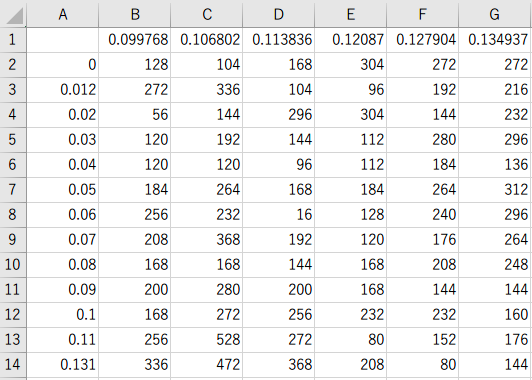
\includegraphics[width=10cm]{./fig/data_table_example.png}
  \caption{得られるデータテーブルの例}
  \label{fig:data_table_example}
\end{figure}

\newpage
\section{Simulinkにデータを転送するMATLABコード}
 SimInを使用してSimulinkに読み込ませる.Simlink側ではfromWorkspaceブロックを使用してデータを取り込む.データは多次元配列として取り込まれる.

\begin{lstlisting}[language=MATLAB]
clc;clear;

%% Setting the import range
start_time = 15;
end_time = 35;

%% Select data to read
select_data = 'test_data/non-LPF-High';

%% Read RADRA data
% Generate matrix data from CSV
radar_raw_data = readmatrix(strcat(select_data, '/3.csv'));
radar_raw_data(end,:) = [];
radar_amp_data = radar_raw_data(2:end,2:end);
radar_time_data = radar_raw_data(2:end,1);
radar_dis_data = radar_raw_data(1,2:end);

%% Read acceleration data
acc_raw_data = readmatrix(strcat(select_data, '/acc.csv'));
acc_raw_data(end,:) = [];
acc_time_data = acc_raw_data(:,1);
acc_data = acc_raw_data(:,2);

%% Generate data for Simulink to read
SimIn = createSimuIn(radar_time_data, radar_amp_data);
Simin_dis = createSimuIn(0, radar_dis_data);
simin_acc = createSimuIn(acc_time_data, acc_data);

%% Draw graph
subplot(2,1,1)
mesh(SimIn.time, radar_dis_data, SimIn.signals.values.')
view(2)
subplot(2,1,2)
plot(radar_dis_data, SimIn.signals.values)
% plot(simin_acc.time, simin_acc.signals.values)

%% Parameters
stopTime = SimIn.time(end);
indexToMeter = radar_dis_data(1, 2) - radar_dis_data(1, 1);

%% Generate SimIn
function SimIn = createSimuIn(times, vals)
    SimIn.signals.values = vals;
    SimIn.signals.dimensions = size(SimIn.signals.values,2);
    SimIn.time = times;
end
\end{lstlisting}

